\documentclass{article}
\usepackage[utf8]{inputenc}
\usepackage{graphicx}
\usepackage{a4wide}
\usepackage{float}
\addtolength{\topmargin}{-1in}
\pagenumbering{gobble}

\title{Are temperatures of one year significantly correlated with the next year (successive years), across years in a given location?}
\author{Kate Griffin, Peter Zeng, Junyue Zhang, Kayleigh Greenwood}
\date{December 2021}

\begin{document}
	
	\maketitle
	
	\section{Introduction}
	A permutation analysis was conducted to investigate whether the temperatures of one year significantly correlated with the next year (successive years) in Florida. Correlation was calculated using data from the annual temperature dataset from Key West in Florida, USA for the 20th century. 
	
	\section{Methods}
	The Pearson's correlation coefficient between the temperature of each year and its successive year was calculated. The temperature values of the successive year was re-sampled to make 1000 permuted samples. The correlation coefficient was calculated between the temperature of that year and permuted temperature values. The fraction of permuted coefficients which were greater than the observed coefficient value was calculated (i.e. the asymptotic p-value). The distribution of permuted samples were visualised on a histogram, with a vertical line representing the observed correlation coefficient. 
	
	\section{Results} 
	There was a significant correlation between temperature and year (p-value=0.001). 
	\begin{figure}[H]
		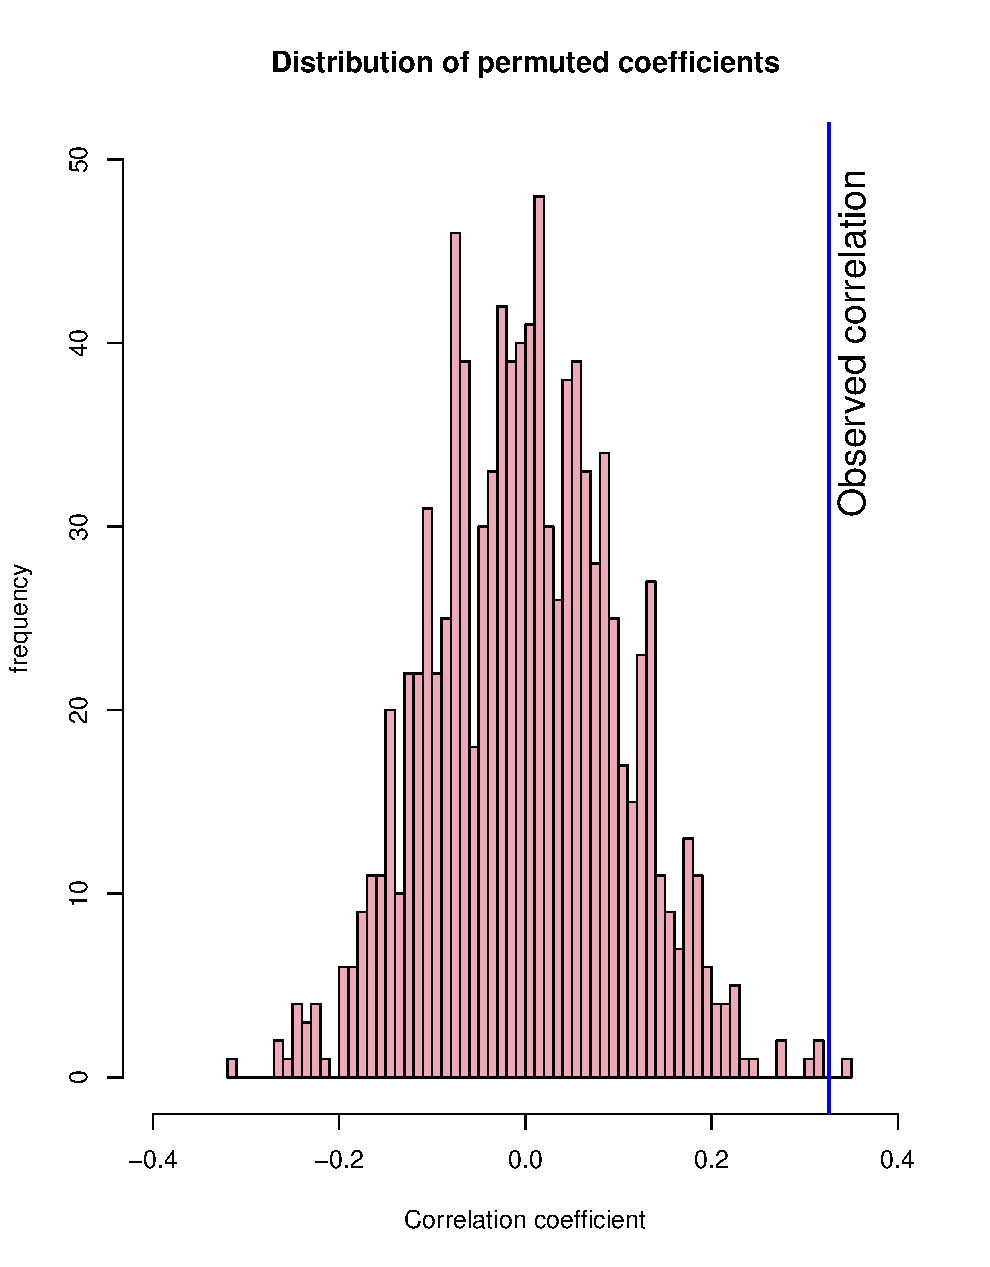
\includegraphics[width= 50 mm, scale=0.31]{../data/TAutoCorr_hist.pdf}
		\caption{The distribution of correlation coefficients of permuted samples. The blue line represents the observed correlation coefficient}
		\label{The distribution of correlation coefficients of permuted samples. The blue line represents the observed correlation coefficient}
	\end{figure}
	
\end{document}